\documentclass[12pt,a4paper]{article}

\usepackage[pdftex]{geometry}
\geometry{lmargin=6em,rmargin=6em,bmargin=6em,tmargin=6em}

\usepackage[pdftex]{graphicx}
\DeclareGraphicsExtensions{.pdf,.png,.jpg}

\title{HiPERCAM timing, version 3}
\author{T.R. Marsh}
\date{\today}

\begin{document}
\maketitle

\section{Introduction}

The per-frame timing data from HiPERCAM comes in 36 bytes packed at the end of
each frame, but this is just the GPS timestamp taken at a particular time in
the exposure cycle, and one needs to correct this time into a time at
mid-exposure. This is potentially different for each CCD because of HiPERCAM's
NSKIP option whereby frame transfers do not take place allowing some CCDs
longer exposures than others. This document specifies how this correction is
carried out.

\section{The exposure sequence}

\subsection{No clear mode}

\begin{figure}
\begin{center}
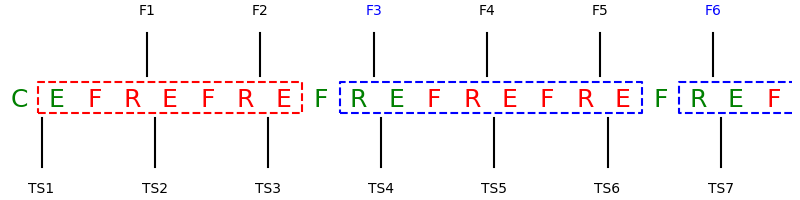
\includegraphics[width=0.95\textwidth]{noclear}
\end{center}
\caption{\label{noclear} The exposure sequence for a CCD with NSKIP set to 2 in
  no clear mode.  The letters stand for: 'C' = clear'; 'W' = wipe; 'E' =
  expose; 'F' = frame-transfer; 'R' = readout; 'D' = data out; 'TS' =
  time-stamp. Those in red are dummy operations, i.e. they appears in the
  sequence as a delay to keep the timing of all CCDs in sync, but nothing
  actually happens (although there is no difference in the case of 'E' the
  exposure delay). The dashed boxes indicate the duration of the
  exposures. The first in red is a special case since it does not include the
  readout of the previous frame unlike all subsequent frames. This one is read
  out as frame 3 (F3) with time stamp 3 (TS3) attached. The next good frame
  enclosed in blue is read out as F6 with TS6 attached.}
\end{figure}

Fig.~\ref{noclear} shows the sequence of events in no clear mode, at the start of
a run, beginning with an initial clear. In the case shown, NSKIP=2, so that
useful data appears every third frame. Thus F3 and F6 are proper data and
appear after a real frame transfer and read, whereas the 5th frame (F5) is
junk data following a read of the masked off area when there was no frame
transfer. F6, which is the first of the 'regular' exposures, unaffected by
end-effects at the start. The exposure upon which it is based is marked by the
blue box. It starts immediately after the (genuine) frame transfer that occurs
after the third time stamp (TS3) is taken. The data moved into the masked area
from this frame transfer appear as F3, but photons accumulate in the imaging
area up to the frame transfer that occurs after TS6. Thus the fundamental
cycle period is 3 = NSKIP + 1.

The mid-exposure time we want in the average of the start and end times. We
reference these with respect to TS6, since that is the time stamp that will be
tacked on to F6 and is the ``per-frame'' timing data referred to earlier.

Adopting an obvious notation, the time of the end of the exposure, $t_2$, is
given by
\[ t_2 = t_S + t_E,\]
while the start is
\[ t_1 = t_S - n_{\mathrm{skip}} (t_F + t_R + t_E) - t_R.\]
The average of these is the time we want, i.e.
\begin{equation}
t_{\mathrm{mid}} = t_S + \left(\frac{t_E - t_R}{2}\right) -
\left(\frac{t_F + t_R + t_E}{2}\right) n_{\mathrm{skip}} ,\label{tmid-norm}
\end{equation}
Here $t_S$ is the timestamp of the frame in question, whiel $t_F$, $t_R$ and 
$t_E$ are the times taken to frame transfer, readout, and the exposure
delay (user defined). Eq.~\ref{tmid-norm} applies
to frame number $(n_{\mathrm{skip}}+1) m$, where $m$ is an integer, $\forall m >
  1$. e.g. in the example, $n_{\mathrm{skip}} = 2$, $m = 2$ gives the time for
  F6. Times are meaningless for any of the dummy frames (F2, F5 etc) since they
  don't contain data, which leaves the $m = 1$ case, F3. The exposure for this
  is high-lighted in red in Fig.~\ref{noclear}. If it is compared to the blue
  box, it can be seen to lack the 'R' stage at the start relative to that,
so we can take Eq.~\ref{tmid-norm} and add $t_R/2$ to get the special
case for the first (non-junk) frame:
\begin{equation}
t_{\mathrm{mid}} = t_S + \frac{t_E}{2} -
\left(\frac{t_F + t_R + t_E}{2}\right) n_{\mathrm{skip}} .\label{tmid-spec}
\end{equation}

Finally the exposure times are
\begin{eqnarray}
t_{\mathrm{exp}} &=& (t_F + t_R + t_E) n_{\mathrm{skip}} + t_R + t_E,\\
t_{\mathrm{exp}} &=& (t_F + t_R + t_E) n_{\mathrm{skip}} + t_E,
\end{eqnarray}
for the normal ($m > 1$) and special ($m = 1$) cases respectively.

\subsection{Clear mode}

\begin{figure}
\begin{center}
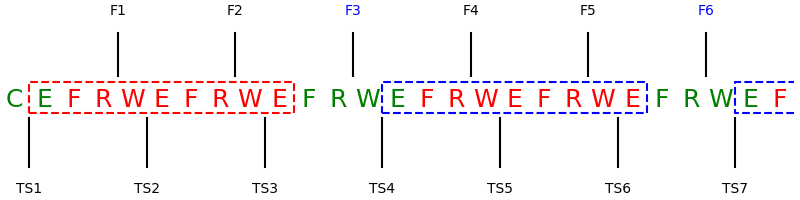
\includegraphics[width=0.95\textwidth]{clear}
\end{center}
\caption{\label{clear} The sequence for clear mode.}
\end{figure}

Fig.~\ref{clear} shows the clear mode case. The difference is that after each
readout there is now a genuine wipe, although with nskip in operation, some of
these are simply short delays to keep synchronisation. That means photons that
accumulated in the imaging area during readout of the masked area are thrown
away, and the exposure only starts once the wipe is completed. This allows
shorter exposures which can be useful on bright objects, although at the cost
of increased deadtime. It is often useful for calibrations. The mid-exposure 
time in this case is given by
\begin{equation}
t_{\mathrm{mid}} = t_S + \frac{t_E}{2} -
\left(\frac{t_F + t_R + t_W + t_E}{2}\right) n_{\mathrm{skip}} ,
\end{equation}
which applies in all cases.
If we define $t_W = 0$ in the no clear case, then this equation also applies
to the first good exposure of no clear mode, and we just need a $-t_R/2$
correction to get the other ones.

Finally, the exposure time in clear mode is given by
\begin{equation}
 t_{\mathrm{exp}} = (t_F + t_R + t_W + t_E) n_{\mathrm{skip}} + t_E.
\end{equation}

The Python class {\tt Times} within {\tt hcam.py} implements these relations.

\subsection{Drift mode}

\begin{figure}
\begin{center}
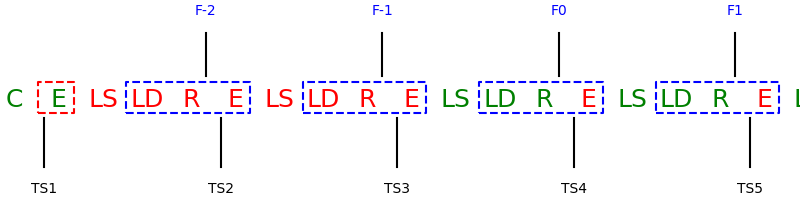
\includegraphics[width=0.95\textwidth]{drift}
\end{center}
\caption{\label{clear} The sequence for drift mode. 'LS' and 'LD' stand for
line-shift and line-dump.}
\end{figure}

In drift mode the windows are partially shifted into the masked area so that
there are one or more of them in the masked area as windows are being read
out. The smaller shifts allow the deadtime between exposures to be reduced.

% t1 = ts - R - LD
% t2 = ts + E
%
% R = ESO DET TREAD
% LD = ESO DRIFT TLINEDUMP
% E = ESO DET TDELAY

The mid-exposure time is given by 
\begin{equation}
t_{\mathrm{mid}} = t_S + t_E + t_{\mathrm{LS}}
+\frac{1}{2} (t_{\mathrm{LD}} + t_R)
\end{equation}
\emph{Not sure about this; it needs checking. It differs
from an e-mail from Stu. Does the photon accumulation really start between
LS and LD as indicated and stop at the start of LS? Don't we need to account
for the number of windows in the masked area?}

\end{document}
